\documentclass{article}
\usepackage[utf8]{inputenc}
\usepackage{geometry}
\usepackage{amsmath}
 \geometry{
 a4paper,
 total={170mm,257mm},
 left=20mm,
 top=20mm,
 }
 \usepackage{graphicx}
 \usepackage{titling}

 \title{Assignment \textbf{3} (Lecture 9-11)
}
\author{Syed Suhaib Ahmad}
\date{\today}
 
 \usepackage{fancyhdr}
\fancypagestyle{plain}{%  the preset of fancyhdr 
    \fancyhf{} % clear all header and footer fields
    
    \fancyfoot[C]{1}
    \fancyhead[L]{8.02x - Electricity and Magnetism}
    \fancyhead[R]{\theauthor}
}
\makeatletter
\def\@maketitle{%
  \newpage
  \null
  \vskip 1em%
  \begin{center}%
  \let \footnote \thanks
    {\LARGE \@title \par}%
    \vskip 1em%
    %{\large \@date}%
  \end{center}%
  \par
  \vskip 1em}
\makeatother

\usepackage{lipsum}  
%\usepackage{cmbright}

\begin{document}

\maketitle


\subsubsection*{Problem 3.1 - Capacitors in series and parallel}
\begin{enumerate}
    \item[(a)]Determine the equivalent capacitance of the circuit
shown in Figure 1.
    \item[(b)]If $C_1=C_2=2C_3=24\mu\,$F, how much charge is store on each capacitor when $V=35.0\,$V?
    \begin{figure}[h]
        \centering
        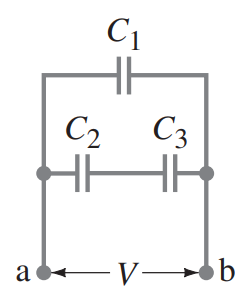
\includegraphics[width=0.2\linewidth]{figs/fig_prob_3.1.png}
        \caption{Capacitors in series and parallel}
        \label{fig: }
    \end{figure}
\end{enumerate}
\textbf{Solution(a)}
\\
\\To find the effective capacitance of the given circuit, we first find the combined capacitance, $C_{23}$, of $C_2$ and $C_3$. Since they are connected in series,
\[\frac{1}{C_{23}}=\frac{1}{C_2}+\frac{1}{C_3}\Rightarrow C_{23}=\left(\frac{1}{C_2}+\frac{1}{C_3}\right)^{-1}.\]
Finally, the equivalent capacitance, $C_{\text{total}}$, of the circuit can be determined by adding $C_{23}$ with $C_1$ as they are connected in parallel.
\[C_{\text{total}}=C_1+\left(\frac{1}{C_2}+\frac{1}{C_3}\right)^{-1}.\]
\textbf{Solution(b)}
\\
\\The charge stored on $C_1$ is relatively straightforward, $Q_1=C_1V=24\times10^{-6}\times35.0=0.84\,$mC.
The potential difference across $C_2$ and $C_3$ is given by the equation
\begin{equation}
    V_2+V_3=V\Rightarrow \frac{Q_2}{C_2}+\frac{Q_3}{C_3}=V.
\end{equation}
Using the law of conservation of charge, it can be concluded that $Q_2=Q_3=Q$. This is because no charge can leave or enter the part of circuit containing the right plate of $C_2$ and left plate of $C_3$. So, if it was neutral initially, the charge on right plate of $C_2$ has to be equal and opposite to the charge on left plate of $C_3$. Hence, (1) now becomes
\[\frac{Q}{C_2}+\frac{Q}{\frac{C_2}{2}}=V\]
\[\frac{\frac{3Q}{2}}{\frac{C_2}{2}}=V\]
\[Q=\frac{C_2V}{3}\]
\[=\frac{24\times10^{-6}\times35.0}{3}\]
\[=0.28\,\text{mC}.\]
\newpage

\subsubsection*{Problem 3.2 - Switching capacitors}
In the diagram below, the four capacitors have the same capacitance; the battery provides $120\,$V.
\begin{figure}[h]
    \centering
    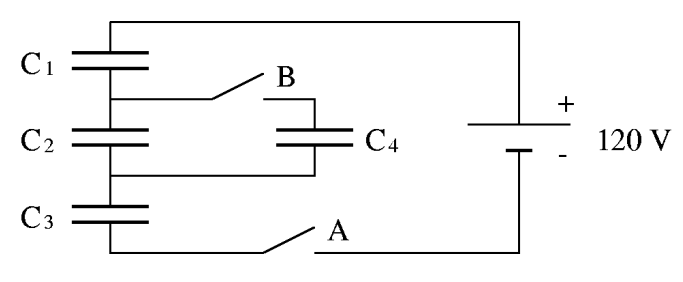
\includegraphics[width=0.5\linewidth]{figs/fig_prob_3.2.png}
    %\caption{Caption}
    %\label{fig:enter-label}
\end{figure}
\\Consider two cases, starting in both cases with uncharged capacitors.
\\
\\\textbf{\textit{Case I:}}
\begin{enumerate}
    \item[(a)]While switch B is kept open, switch A is closed and then opened after $C_1$, $C_2$, and $C_3$ are fully charged. What is now the electric potential difference across each capacitor?
    \item[(b)]Subsequently, switch B is closed. What is now the electric potential difference across each capacitor?
\end{enumerate}
\textbf{\textit{Case II:}}
\begin{enumerate}
    \item[(c)]Switch A is open. Switch B is first closed. What is now the electric potential difference across each capacitor?
    \item[(d)]Subsequently switch A is closed. What is now the potential difference across each capacitor?
\end{enumerate}
\textbf{Solution(a)}
\\
\\
Since, in this arrangement, all three of the capacitors are connected in series; the potential difference across each capacitor must satisfy the equation
\[V_1+V_2+V_3=120\,.\]
However, $Q_1=Q_2=Q_3=Q$, this is because of the fact that each of these capacitors have the same capacitance and a current $I$ passes through each of them, thus charge conservation also supports this argument.
\[Q=CV_1=CV_2=CV_3\Rightarrow V_1=V_2=V_3=40\,\text{V}.\]
\textbf{Solution(b)}
\\
\\Potential difference will remain the same across each capacitor once all of them are charged regardless of weather the switch A is opened or closed. However, now a new capacitor, $C_4$, has been added to the circuit. As switch A is opened so no charge can escape from $C_1$ and $C_3$ and due to the addition of $C_4$, the charge on $C_2$ will distribute equally between $C_2$ and $C_4$. Since $C_2=C_4$, and due to the same conclusions made in part (a), $Q_2=Q_4\Rightarrow CV_2=CV_4\Rightarrow V_2=V_4=20\,\text{V}$. 
\\
\\\textbf{Solution(c)}
\\
\\This would have no effect on the state of each capacitor as all of them are initially uncharged and closing switch B only means the battery is disconnected.
\\
\\\textbf{Solution(d)}
\\
\\For this particular scenario, the effective capacitance of the circuit can be written as
\[C_T=\left(\frac{1}{C_1}+\frac{1}{C_2+C_4}+\frac{1}{C_3}\right)^{-1}=\left(\frac{1}{C}+\frac{1}{2C}+\frac{1}{C}\right)^{-1}=\frac{2}{5}C\,.\]
Total charge drawn from the battery onto all the capacitors is $Q_T=\frac{2}{5}CV$\,.
Now potential difference across each of the capacitors can be determined as follows
\[V_1=V_3=\frac{Q_T}{C}=\frac{2}{5}\times120=48\,\text{V}\,.\]
\[V_2=V_4=\frac{Q_T}{2C}=\frac{1}{5}\times120=24\,\text{V}\,.\]

\newpage

\subsubsection*{Problem 3.3 - The effect of a dielectric medium on the capacitance}
A slab of width $d$ and dielectric constant $K$ is inserted
a distance $x$ into the space between the square parallel
plates (of side \textit{l}) of a capacitor. Determine, as a function of $x$,
\begin{enumerate}
    \item[(a)]the capacitance,
    \item[(b)]the energy stored if the potential difference is $V_0$, and
    \item[(c)]the magnitude and direction of the force exerted on the slab (assume $V_0$ is constant).
    \begin{figure}[h]
    \centering
    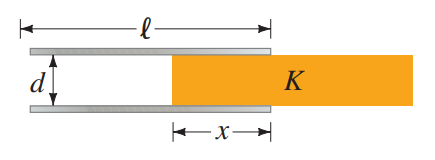
\includegraphics[width=0.4\linewidth]{figs/fig_prob_3.3.png}
  %  \caption{}
 %   \label{Figure 2}
\end{figure}
\end{enumerate}
\textbf{Solution(a)}
\\
\\We approach this problem by considering two regions, one with dielectric constant of 1 and the other with dielectric constant $K$. For simplicity, we assume both regions are capacitors connected in parallel. Capacitance of a parallel plate capacitor is $\frac{\epsilon_0A}{d}$, the area of both regions is $l(l-x)$ and $lx$. Thus the total capacitance is
\[C_T=C_1+C_2=\frac{\epsilon_0l(l-x)}{d}+\frac{K\epsilon_0lx}{d}=\frac{\epsilon_0l}{d}\left[l+x(K-1)\right].\]
\textbf{Solution(b)}
\\
\\Energy stored in the entire system is given by
\[U=\frac{1}{2}C_TV_0^2=\frac{\epsilon_0lV_0^2}{2d}\left[l+x(K-1)\right].\]
\textbf{Solution(c)}
\\
\\Initially the capacitance of the capacitor is $\frac{\epsilon_0l^2}{d}$. Upon moving a dielectric material a distance $\Delta x$ in between the plates changes the capacitance to $\frac{\epsilon_0l}{d}[l+\Delta x(K-1)]$ as we saw in part (a). Since $K>1$, there has been an increase in the capacitance and thus the energy stored has also increased (as $V_0$ is constant).
\[\Delta U=\frac{1}{2}C_{\text{final}}V_0^2-\frac{1}{2}C_{\text{initial}}V_0^2=\frac{V_0^2\epsilon_0l}{2d}[l+\Delta x(K-1)]-\frac{V_0^2\epsilon_0l^2}{2d}=\frac{V_0^2\epsilon_0l}{2d}\Delta x(K-1).\]
We know that electric field inside the capacitor has decreased as $E_{\text{new}}=\frac{E_{\text{free}}}{K}$, where $E_{\text{free}}$ is the original electric field without dielectric material. However, since distance $d$ and potential difference $V_0$ have remained constant, $E_{\text{new}}$ cannot be less than $\frac{V_0}{d}$. To tackle this problem, battery does work, $W_{\text{battery}}$, to accumulate more charge on the capacitor increasing $E_{\text{free}}$. Therefore,
\[\Delta Q=V_0C_\text{final}-V_0C_{\text{initial}}=\frac{V_0\epsilon_0l}{d}[l+\Delta x(K-1)]-\frac{V_0\epsilon_0l^2}{d}=\frac{V_0\epsilon_0l}{d}\Delta x(K-1).\]
This gives
\[W_{\text{battery}}=\Delta QV_0=\frac{V_0^2\epsilon_0l}{d}\Delta x(K-1).\]
Work required to insert the dielectric in between the plates is $W_{\text{insert}}$. Thus, the total energy change in this process can be summarized in the equation below.
\[\Delta U=W_{\text{battery}}+W_{\text{insert}}\Rightarrow W_{\text{insert}}=\Delta U-W_{\text{battery}}\]
This work, $W_{\text{insert}}$, in inserting the dielectric a distance $\Delta x$ is equal to $F_{\text{insert}}\Delta x=-F_{\text{electrical}}\Delta x$.
\[F_{\text{electrical}}=-\frac{\Delta U-W_{\text{battery}}}{\Delta x}=-\frac{\frac{V_0^2\epsilon_0l}{2d}\Delta x(K-1)-\frac{V_0^2\epsilon_0l}{d}\Delta x(K-1)}{\Delta x}=\frac{V_0^2\epsilon_0l}{2d}(K-1).\]
Positive nature of $F_{\text{electrical}}$ indicates that slab is pulled inwards by this electrical force.


\subsubsection*{Problem 3.4 - Comparing cylindrical and spherical capacitors}
\begin{enumerate}
    \item[(a)]Compare the capacitance of a capacitor of 2 concentric shapes with $R_1=6\,$cm and $R_2=9\,$cm, with that of a cylindrical capacitor having the same radii and axial length $15\,$cm. Why are the capacitance values nearly equal? 
    \item[(b)]Show that, when $R_1$ and $R_2$ are nearly equal ($R_2=R_1+\delta;\delta<<R_1$) the formulas for the spherical and cylindrical capacitors may be approximated by the formula for the parallel-plate capacitor, $C=\epsilon_0A/d$.
    \textit{Hint: make use of Taylor's expansion in terms of $\delta/R_1$.}
\end{enumerate}
\textbf{Solution(a)}
\\
\\To determine the capacitance of a capacitor in form of 2 concentric shapes, we first find the potential difference between them. The electric due to either of the shapes is given by $\frac{Q}{4\pi\epsilon_0R^2}$ (from Gauss's Law). 
\[\Delta V=\int_{0.06}^{0.09}\frac{Q}{4\pi\epsilon_0R^2}\,dR=\frac{Q}{4\pi\epsilon_0}\left[-\frac{1}{R}\right]_{0.06}^{0.09}=\frac{25Q}{18\pi\epsilon_0}.\]
Thus, the capacitance of the sphere is
\[C_{\text{sph}}=\frac{Q}{\Delta V}=\frac{18\pi\epsilon_0}{25}\approx2\times10^{-11}\,\text{F}.\]
Using the same approach as above, we first find the potential difference between the cylinders ($E=\frac{Q}{2\pi\epsilon_0Rl}$ from Gauss's Law)
\[\Delta V=\int_{0.06}^{0.09}\frac{Q}{2\pi\epsilon_0Rl}\,dR=\frac{Q}{2\pi\epsilon_0l}\left[\ln R\right]_{0.06}^{0.09}=\frac{Q}{2\pi\epsilon_0l}\ln\left(\frac{3}{2}\right).\]
Therefore, the capacitance is
\[C_{\text{cyl}}=\frac{Q}{\Delta V}=\frac{2\pi\epsilon_0\times0.15}{\ln(3/2)}\approx2.06\times10^{-11}\,\text{F}.\]
Both capacitance values are approximately equal due to the fact that in both systems, the separation between the plates is same and the plate areas are also nearly equal.
\\
\\\textbf{Solution(b)}
\\
\\Capacitance of the sphere is given by
\[C_{\text{sph}}=4\pi\epsilon_0\left(\frac{R_1R_2}{R_2-R_1}\right)=4\pi\epsilon_0\left(\frac{R_1(R_1+\delta)}{\delta}\right)=\frac{4\pi\epsilon_0R_1^2}{\delta}\left(1+\frac{\delta}{R_1}\right).\]
Since $\delta<<R_1$, the above expression can be approximated to
\[\frac{4\pi\epsilon_0R_1^2}{\delta}=\frac{\epsilon_0A}{\delta}\]
where $A=4\pi R_1^2$, hence this new expression is same as the general formula for capacitance between two parallel plates: $C=\frac{\epsilon_0A}{d}$.
The capacitance of the cylindrical capacitor is
\[C_{\text{cyl}}=\frac{2\pi\epsilon_0l}{\ln(R_2/R_1)}=\frac{2\pi\epsilon_0l}{\ln\left(1+\delta/R_1\right)}\]
The term $\ln(1+\delta/R_1)$ can be approximated to $\delta/R_1$. Hence now $C_{\text{cyl}}$ becomes
\[\frac{2\pi\epsilon_0R_1l}{\delta}=\frac{\epsilon_0A}{\delta}\]
where $A=2\pi R_1l$ is the area of one of the cylindrical shells. Therefore, we have again found that regardless of the geometry of the capacitor, whenever the separation between the plates is very small, the capacitance is approximately the same as the capacitance of a parallel plate capacitor.

\subsubsection*{Problem 3.5 - The Van de Graaff}
The spherical dome of a Van de Graaff electrostatic generator has a radius of $R\,$m. A rubberized belt $50\,$cm wide travels at a velocity of $30\,$m/sec. The belt is given a surface charge density which produces a field of approximately $10^6\,$V/m on each side of the belt.  
\begin{enumerate}
    \item[(a)]What is the current carried by the belt?
    \item[(b)]What is the maximum charge that the spherical dome can hold, and how long will it take to reach this value?
    \item[(c)]What is the maximum electrostatic potential of the spherical dome?
    \item[(d)]What are your answers under (b) and (c) for $R=0.15\,$ and $R=0.5\,$m?
\end{enumerate}
\textbf{Solution(a)}
\\
\\Gauss's Law can be used to show that the electric field outside the belt is given by $E=\frac{\sigma}{2\epsilon_0}$. Thus, now we can calculate the surface charge density of the belt.
\[E=\frac{\sigma}{2\epsilon_0}\Rightarrow\sigma=2\epsilon_0E=2\times8.85\times10^{-12}\times10^6=1.77\times10^{-5}\,\text{C/m}^2.\]
Belt travels a distance of $v\,dt$ in a time interval of $dt$\,s and hence an area of $wv\,dt$ in the same interval. This area contains a charge $dQ=\sigma wv\,dt$ and current is defined as $I=\frac{dQ}{dt}$, therefore
\[I=\frac{d}{dt}(\sigma wv\,dt)=\sigma wv=1.77\times10^{-5}\times0.5\times30\approx2.7\times10^{-4}\,\text{A}.\]
\textbf{Solution(b)}
\\
\\The sphere will hold a maximum charge $Q_{\text{max}}$, when its electric field is equal to the breakdown electric field, $E_{\text{max}}=3\times10^6\,$V/m.
\[E_{\text{max}}=\frac{Q_{\text{max}}}{4\pi\epsilon_0R^2}\Rightarrow Q_{\text{max}}=4\pi\epsilon_0R^2E_{\text{max}}=R^2\left(4\pi\times8.85\times10^{-12}\times3\times10^6\right)=R^2(3.3\times10^{-4})\,\text{C}.\]
If the spherical dome is being charged at a rate of $2.7\times10^{-4}\,$C/s, then the time required to accumulate $Q_{\text{max}}$ would be
\[t_{\text{charge}}=\frac{R^2(3.3\times10^{-4})}{2.7\times10^{-4}}\approx R^2(1.2)\,\text{s}.\]
\textbf{Solution(c)}
\\
\\Maximum electric potential potential is given by
\[V_{\text{max}}=E_{\text{max}}R=R(3\times10^6)\,\text{V}.\]
\textbf{Solution(d)}
\\
\\For $R=0.15\,$m:
\[E_{\text{max}}=(0.15)^2(3.3\times10^{-4})\approx7.4\times10^{-6}\,\text{C}.\]
\[t_{\text{charge}}=\frac{7.425\times10^{-6}}{2.7\times10^{-4}}\approx0.03\,\text{s}.\]
\[V_{\text{max}}=0.15\times3\times10^6=4.5\times10^5\,\text{V}.\]
For $R=0.5\,$m:
\[E_{\text{max}}=(0.5)^2(3.3\times10^{-4})\approx8.3\times10^{-5}\,\text{C}.\]
\[t_{\text{charge}}=\frac{8.25\times10^{-5}}{2.7\times10^{-4}}\approx0.3\,\text{s}.\]
\[V_{\text{max}}=0.5\times3\times10^6=1.5\times10^6\,\text{V}.\]

\newpage

\subsubsection*{Problem 3.6 - Resistor Circuit}
Determine the magnitudes and directions of the currents through $R_1$ and $R_2$ in Figure 2.
\begin{figure}[h]
    \centering
    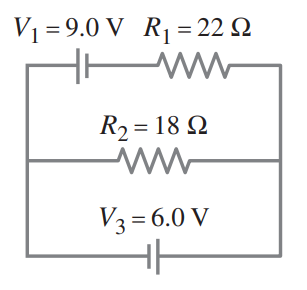
\includegraphics[width=0.25\linewidth]{figs/fig_prob_3.6.png}
    \caption{}
    \label{fig:enter-label}
\end{figure}
\\
\\\textbf{Solution(a)}
\\
\\Going around the outer boundary of circuit in anticlockwise direction gives
\[+V_3-I_1R_1+V_1=0\Rightarrow I_1=\frac{V_3+V_1}{R_1}=\frac{6+9}{22}=0.68\,\text{A}.\]
Similarly, we can do the same for the inner circuit involving $R_2$ and $V_3$:
\[-I_2R_2+V_3=0\Rightarrow I_2=\frac{V_3}{R_2}=\frac{6}{18}=0.33\,\text{A}.\]
Hence, there are currents 0.68 and 0.33\,A in $R_1$ and $R_2$ respectively. Both currents are to the left.

\subsubsection*{Problem 3.7 - Resistor Network}
A circuit consists of 5 resistors and 3 batteries (see diagram); the connecting wires have all a negligible resistance. The values for $R_1, R_2, R_3, R_4$, and $R_5$ are $10\,\Omega, 30\,\Omega, 50\,\Omega, 70\,\Omega$, and $100\,\Omega$, respectively. The batteries have a negligible internal resistance; their voltages $V_1, V_2$, and $V_3$, are $12\,V, 24\,V,$ and $36\,V$, respectively (for their polarities, see the diagram).
\begin{figure}[h]
    \centering
    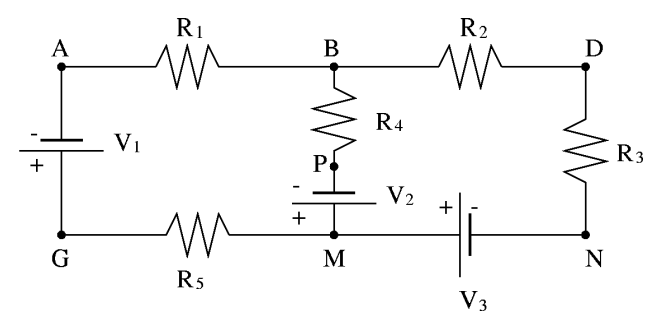
\includegraphics[width=0.5\linewidth]{figs/fig_prob_3.7.png}
%    \caption{Caption}
 %   \label{fig:enter-label}
\end{figure}
 \begin{enumerate}
     \item[(a)]Calculate the current (magnitude and direction) of the currents through each of the 5 resistors.
     \item[(b)]What is the potential difference (observe signs!) between the points A\&P, P\&N, and G\&D.
 \end{enumerate}
 \textbf{Solution(a)}
 \\
 \\We divide the circuit into two parts, one containing; $R_1$, $V_1$, $R_5$, $V_2$, and $R_4$, and the other consisting of; $R_2$, $R_3$, $V_3$, $V_2$, and $R_4$. Moving around the first part in anticlockwise direction gives
 \[+V_1-I_1R_5-V_2-(I_1+I_2)R_4-I_1R_1=0\Rightarrow I_2R_4+I_1(R_5+R_1+R_4)=V_1-V_2\Rightarrow 70I_2+180I_1=-12\]
 and for the second part in same direction
 \[-I_2R_2-I_2R_3+V_3-V_2-(I_1+I_2)R_4=0\Rightarrow I_1R_4+I_2(R_2+R_3+R_4)=V_3-V_2\Rightarrow 70I_1+150I_2=12.\]
 Solving these two equations simultaneously results in
 \[I_1\approx-0.119\,\text{A}\,\,\,\,\,\text{and}\,\,\,\,\,\,I_2\approx0.136\,\text{A}.\]
 Negative nature of $I_1$ suggests that $I_1$ flows in clockwise direction. Thus, current through each of the resistor is
 \[R_1,\,R_5: 119\,\text{mA, clockwise}\,\,\,\,\,\,\,\,\,\,R_2,\,R_3: 136\,\text{mA, clockwise}\,\,\,\,\,\,\,\,\,\,R_4: 16.3\,\text{mA, upwards}.\]
 \textbf{Solution(b)}
 \\
 \\Potential drop across each of the points mentioned in problem is given by:
 \[\Delta V_{AP}=V_A-V_P=(119\times10^{-3}\times10)-(16.3\times10^{-3}\times70)=0.049\,\text{V}\]
 \[\Delta V_{PN}=V_P-V_N=36-24=12\,\text{V}\]
 \[\Delta V_{GD}=(-119\times10^{-3}\times100)+36+(-136\times10^{-3}\times50)=17.3\,\text{V}.\]

\subsubsection*{Problem 3.8 - Wire resistance}
A 5.80-m length of 2.0-mm-diameter wire carries a 
750-mA current when 22.0\,mV is applied to its ends. If the
drift velocity is $1.7\times10^{-5}\,$m/s, determine
\begin{enumerate}
    \item[(a)]the resistance $R$ of the wire,
    \item[(b)]the resistivity $\rho$,
    \item[(c)]the current density $j$,
    \item[(d)] the electric field inside the wire, and 
    \item[(e)] the number $n$ of free electrons per unit volume.
\end{enumerate}
\textbf{Solution(a)}
\\
\\Resistance can be easily calculated using the Ohm's Law.
\[R=\frac{V}{I}=\frac{22}{750}=0.0293\,\Omega=29.3\,\text{m}\Omega.\]
\textbf{Solution(b)}
\\
\\Applying the general relation between resistance, length and cross-sectional area,
\[R\propto\frac{l}{A}\Rightarrow R=\frac{\rho l}{A}\Rightarrow\rho=\frac{RA}{l}=\frac{0.02933\times\pi\times(10^{-3})^2}{5.80}\approx1.6\times10^{-8}\,\Omega\text{m}.\]
\textbf{Solution(c)}
\\
\\Current density is given by
\[j=\frac{I}{A}=\frac{750\times10^{-3}}{\pi\times(10^{-3})^2}\approx2.39\times10^5\,\text{Am}^{-2}.\]
\textbf{Solution(d)}
\\
\\The electric field inside a wire is simply the product of its resistivity and current density.
\[E=\rho j=1.6\times10^{-8}\times2.39\times10^5\approx3.8\times10^{-3}\,\text{Vm}^{-1}.\]
\textbf{Solution(e)}
\\
\\Number of free electrons per unit volume or the number density of the electrons is given by
\[n=\frac{I}{Av_dq}=\frac{750\times10^{-3}}{\pi\times(10^{-3})^2\times1.7\times10^{-5}\times1.6\times10^{-19}}\approx8.8\times10^{28}\,\text{electrons/m}^3.\]

\subsubsection*{Problem 3.9 - Energy consumption of heater}
\begin{enumerate}
    \item[(a)]A particular household uses a 1.8-kW heater 2.0\,h/day (“on” time), four 100-W lightbulbs 6.0\,h/day a 3.0-kW electric stove element for a total of 1.0\,h/day, and miscellaneous power amounting to 2.0\,kWh/day. If electricity costs \$0.105 per kWh, what will be their monthly bill (30\,d)?
    \item[(b)] How much coal (which produces 7500\,kcal/kg) must be burned by a 35\%-efficient power plant to provide the yearly needs of this household?
\end{enumerate}
\textbf{Solution(a)}
\\
\\Total energy consumption per day:
\[2(1.8)+4(0.1\times6)+3+2=11\,\text{kWh}.\]
Hence, monthly bill of this household is
\[11\times30\times0.105\approx35\,\text{\$}.\]
\textbf{Solution(b)}
\\
\\Total energy consumption per year of the household:
\[11\times365=4015\,\text{kWh}=1.4454\times10^{10}\,\text{J}.\]
In general, total coal required to meet this consumption is (1\,kcal=4184\,\text{J})
\[\frac{1.4454\times10^{10}}{7500\times4184}\approx460\,\text{kg}.\]
Since the power plant produces coal at 35\% efficiency, total coal required to give 460 kilograms is 
\[\frac{460}{0.35}\approx1300\,\text{kg}.\]

\subsubsection*{Problem 3.10 - Electric car}
A proposed electric vehicle makes use of storage batteries as its source of energy. Its mass is 1560\,kg and it is powered by 24 batteries, each 12\,V, 95\,A$\cdot$h. Assume that the car is driven on level roads at an average speed of 45\,km/h and the average friction force is 240\,N. Assume 100\% efficiency and neglect energy used for acceleration. No energy is consumed when the vehicle is stopped, since the engine doesn’t need to idle.
\begin{enumerate}
    \item[(a)]Determine the horsepower required.
    \item[(b)]After approximately how many kilometers must the batteries be recharged?
\end{enumerate}
\textbf{Solution(a)}
\\
\\Since there is a frictional force of 240\,N, the car's engine must provide a driving force to tackle this opposing force. Thus, the minimum power required by the engine is
\[P=Fv=240\times\frac{45\times10^3}{3600}=3000\,\text{W}\approx4.1\,\text{horsepower}.\]
\textbf{Solution(b)}
\\
\\Total energy stored in the batteris when they are fully charged:
\[E=24\times12\times95=27360\,\text{Wh}=9.85\times10^7\,\text{J}.\]
Work done by the batteries in moving the car by a distance $d$ in one charge is
\[E=Fd\Rightarrow9.85\times10^7=240\times d\Rightarrow d=\frac{9.85\times10^7}{240}=410.4\,\text{km}.\]

\end{document}
